\section<presentation>[Impl�mentation]{Impl�mentation}
  \begin{frame}
    \frametitle{Organisation du programme}
      Le programme contient :
      \begin{itemize}
        \item un \texttt{README} tr�s complet ;
        \item un r�pertoire base, regroupant plusieurs librairies externes (sous licences compatibles GPLv2) ;
        \item un fichier de configuration ;
        \item \texttt{queue.h/cc}, \texttt{packet.h/cc} et \texttt{conntrack.h/cc} qui r�alisent l'interception des paquets envoy�s �
        \texttt{NFQUEUE} (\texttt{queue.cc}), leur interpr�tation (\texttt{packet.cc}), et leur mise en relation avec un conntrack
        (\texttt{conntrack.cc}) ;
        \item \texttt{classifier.h/cc} qui sert � classer les paquets ;
        \item un fichier de base permettant le lancement des threads, un autre parsant le fichier de configuration et
        initialisant le classifier.
      \end{itemize}
  \end{frame}

  \begin{frame}
    \frametitle{Fonctionnement du logiciel}
      \begin{itemize}
        \item<1-> Regrouper les paquets appartenant � une m�me connexion, gr�ce � l'utilisation de
        \texttt{libnetfilter\_conntrack};
        \item<2-> D�terminer si le contenu de la connexion correspond � un protocole support�;
        \item<3-> Extraire la m�thode et l'url utilis�es par le client des paquets;
        \item<4-> Classifier et remonter l'information au noyau.
      \end{itemize}
  \end{frame}

  \begin{frame}
    \frametitle{Fonctionnement du logiciel}
      \begin{figure}[h]
        \centering
        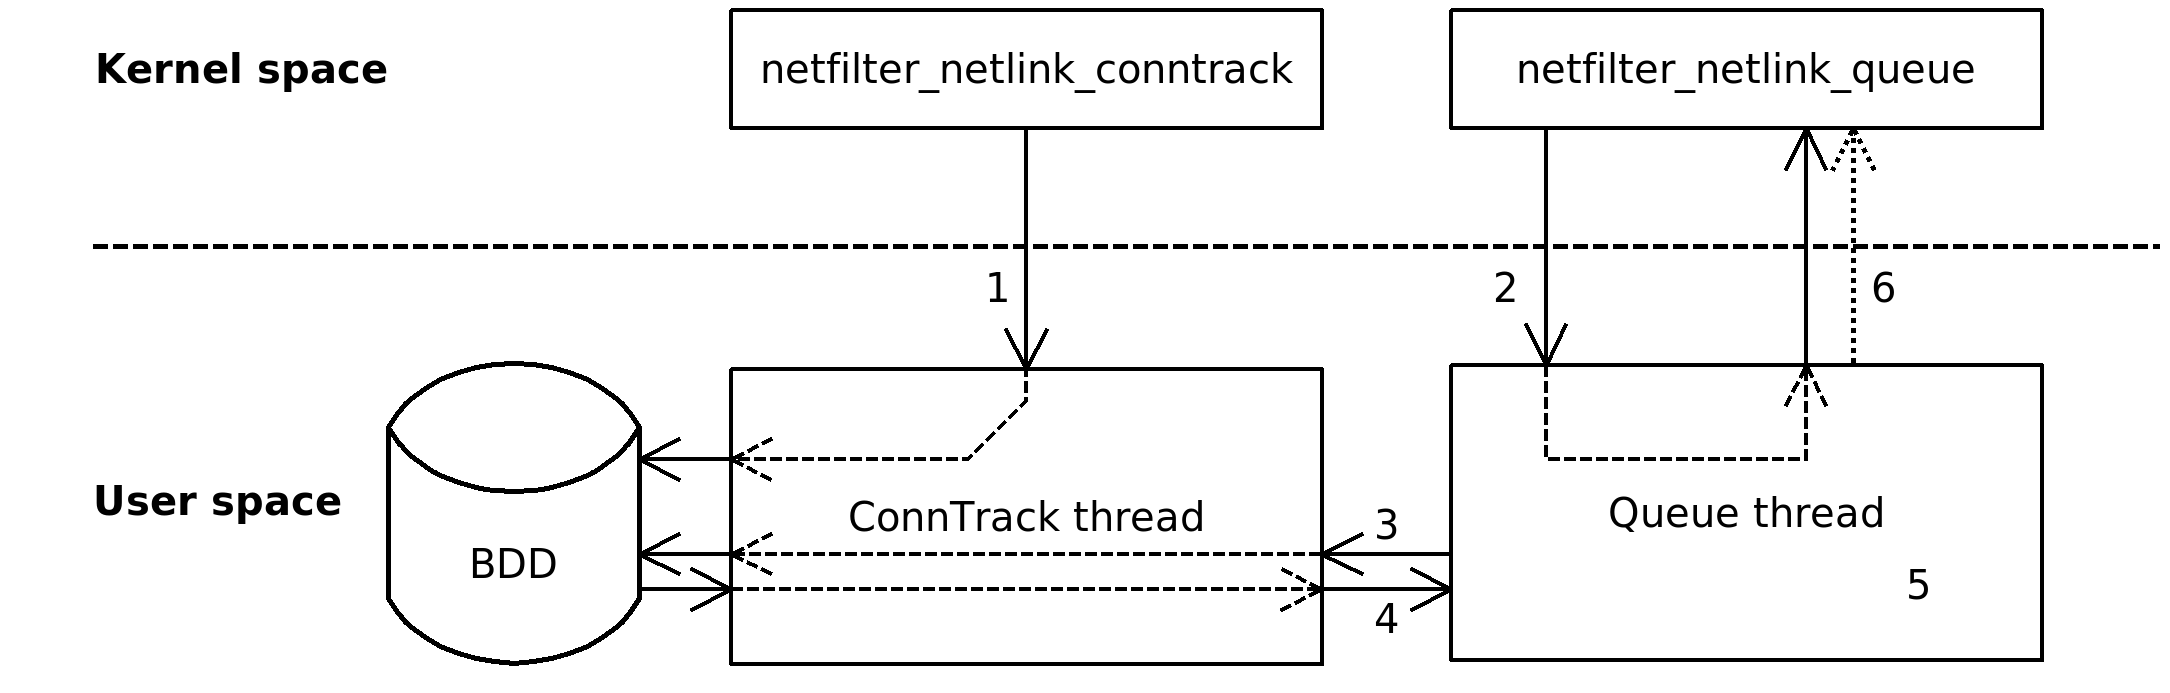
\includegraphics[width=\textwidth]{schema2.png}\\
        \title{Fonctionnement du module}
      \end{figure}
  \end{frame}

  \begin{frame}
    \frametitle{Fonctionnement pratique}
      \begin{itemize}
        \item<1-> Le 1\ier{} thread �coute sur un \texttt{netfilter\_netlink}, re�oit les mises � jour de la table conntrack du
        noyau et maintient une copie locale.
        \item<2-> Le 2\ieme{} thread intercepte les paquets arrivant sur une
        \texttt{NFQUEUE}, les parse, d�termine l'entr�e conntrack et r�cup�re l'objet \og Connection \fg{}
        correspondant, met � jour les deux buffers, puis appelle la m�thode \texttt{update} du classifier avant d'accepter le
        paquet, en le marquant.
        \item<3-> Le classifier surveille les buffers d'une connexion et prend une d�cision.
      \end{itemize}
  \end{frame}

  \begin{frame}
    \frametitle{Fiabilit� et limitation}
      \begin{itemize}
        \item<1-> Le protocole ftp est g�r� correctement.
        \item<2-> Les requ�tes en \emph{Keep-Alive} dans l'http ne sont pas g�r�es.
        \item<3-> L'application r�siste nativement aux attaques de types \emph{Denial of Service}.
      \end{itemize}
  \end{frame}
